\documentclass[
% -- opções da classe memoir --
12pt,				% tamanho da fonte
openright,			% capítulos começam em pág ímpar (insere página vazia caso preciso)
twoside,			% para impressão em recto e verso. Oposto a oneside
a4paper,			% tamanho do papel. 
% -- opções da classe abntex2 --
%chapter=TITLE,		% títulos de capítulos convertidos em letras maiúsculas
%section=TITLE,		% títulos de seções convertidos em letras maiúsculas
%subsection=TITLE,	% títulos de subseções convertidos em letras maiúsculas
%subsubsection=TITLE,% títulos de subsubseções convertidos em letras maiúsculas
% -- opções do pacote babel --
english,			% idioma adicional para hifenização
french,				% idioma adicional para hifenização
spanish,			% idioma adicional para hifenização
brazil				% o último idioma é o principal do documento
]{abntex2}

% ---
% Pacotes básicos 
% ---
\usepackage{lmodern}			% Usa a fonte Latin Modern			
\usepackage[T1]{fontenc}		% Selecao de codigos de fonte.
\usepackage[utf8]{inputenc}		% Codificacao do documento (conversão automática dos acentos)
\usepackage{indentfirst}		% Indenta o primeiro parágrafo de cada seção.
\usepackage{color}				% Controle das cores
\usepackage{graphicx}			% Inclusão de gráficos
\usepackage{microtype} 			% para melhorias de justificação
% ---

% ---
% Pacotes adicionais, usados apenas no âmbito do Modelo Canônico do abnteX2
% ---
\usepackage{lipsum}				% para geração de dummy text
% ---

% ---
% Pacotes de citações
% ---
\usepackage[brazilian,hyperpageref]{backref}	 % Paginas com as citações na bibl
\usepackage[alf]{abntex2cite}	% Citações padrão ABNT

% --- 
% CONFIGURAÇÕES DE PACOTES
% ---

% Configurações do pacote backref
% Usado sem a opção hyperpageref de backref
\renewcommand{\backrefpagesname}{Citado na(s) página(s):~}
% Texto padrão antes do número das páginas
\renewcommand{\backref}{}
% Define os textos da citação
\renewcommand*{\backrefalt}[4]{
	\ifcase #1 %
	Nenhuma citação no texto.%
	\or
	Citado na página #2.%
	\else
	Citado #1 vezes nas páginas #2.%
	\fi}%
% ---

% ---
% Informações de dados para CAPA e FOLHA DE ROSTO
% ---
\titulo{Projeto Integrado de Extensão I}
\autor{BS Beauty Academy}
\local{São Paulo, SP - Brasil}
\data{2025}
\orientador{Marcelo Tavares}
\instituicao{%
	Instituto Federal de Educação, Ciência e\\ Tecnologia de São Paulo -- IFSP
	\par
	Tecnologia em Análise e Desenvolvimento de Sistemas
	\par
	Programa de graduação}
\tipotrabalho{Projeto Integrado de Extensão}
% O preambulo deve conter o tipo do trabalho, o objetivo, 
% o nome da instituição e a área de concentração 
\preambulo{Este projeto integrado de extensão, desenvolvido como parte do curso de Tecnologia em Análise e Desenvolvimento de Sistemas do Instituto Federal de Educação, Ciência e Tecnologia de São Paulo, tem como objetivo desenvolver uma aplicação para otimizar a gestão e o agendamento de serviços de um salão de beleza organizado como um espaço "co-working". A área de concentração do projeto é a inovação tecnológica aplicada ao setor de serviços de beleza.}
% ---

% Configurações de aparência do PDF final

% alterando o aspecto da cor azul
\definecolor{blue}{RGB}{41,5,195}

% informações do PDF
\makeatletter
\hypersetup{
	%pagebackref=true,
	pdftitle={\@title}, 
	pdfauthor={\@author},
	pdfsubject={\imprimirpreambulo},
	pdfcreator={LaTeX with abnTeX2},
	pdfkeywords={abnt}{latex}{abntex}{abntex2}{trabalho acadêmico}, 
	colorlinks=true,       		% false: boxed links; true: colored links
	linkcolor=blue,          	% color of internal links
	citecolor=blue,        		% color of links to bibliography
	filecolor=magenta,      		% color of file links
	urlcolor=blue,
	bookmarksdepth=4
}
\makeatother
% --- 

% ---
% Posiciona figuras e tabelas no topo da página quando adicionadas sozinhas
% em um página em branco. Ver https://github.com/abntex/abntex2/issues/170
\makeatletter
\setlength{\@fptop}{5pt} % Set distance from top of page to first float
\makeatother
% ---

% ---
% Possibilita criação de Quadros e Lista de quadros.
% Ver https://github.com/abntex/abntex2/issues/176
%
\newcommand{\quadroname}{Quadro}
\newcommand{\listofquadrosname}{Lista de quadros}

\newfloat[chapter]{quadro}{loq}{\quadroname}
\newlistof{listofquadros}{loq}{\listofquadrosname}
\newlistentry{quadro}{loq}{0}

% configurações para atender às regras da ABNT
\setfloatadjustment{quadro}{\centering}
\counterwithout{quadro}{chapter}
\renewcommand{\cftquadroname}{\quadroname\space} 
\renewcommand*{\cftquadroaftersnum}{\hfill--\hfill}

\setfloatlocations{quadro}{hbtp} % Ver https://github.com/abntex/abntex2/issues/176
% ---

% --- 
% Espaçamentos entre linhas e parágrafos 
% --- 

% O tamanho do parágrafo é dado por:
\setlength{\parindent}{1.3cm}

% Controle do espaçamento entre um parágrafo e outro:
\setlength{\parskip}{0.2cm}  % tente também \onelineskip

% ---
% compila o indice
% ---
\makeindex
% ---

% ----
% Início do documento
% ----
\begin{document}
	
	% Seleciona o idioma do documento (conforme pacotes do babel)
	%\selectlanguage{english}
	\selectlanguage{brazil}
	
	% Retira espaço extra obsoleto entre as frases.
	\frenchspacing 
	
	% ----------------------------------------------------------
	% ELEMENTOS PRÉ-TEXTUAIS
	% ----------------------------------------------------------
	% \pretextual
	
	% ---
	% Capa
	% ---
	\imprimircapa
	% ---
	
	% ---
	% Folha de rosto
	% (o * indica que haverá a ficha bibliográfica)
	% ---
	\imprimirfolhaderosto*
	% ---
	
	% ---
	% Inserir a ficha bibliografica
	% ---
	
	% Isto é um exemplo de Ficha Catalográfica, ou ``Dados internacionais de
	% catalogação-na-publicação''. Você pode utilizar este modelo como referência. 
	% Porém, provavelmente a biblioteca da sua universidade lhe fornecerá um PDF
	% com a ficha catalográfica definitiva após a defesa do trabalho. Quando estiver
	% com o documento, salve-o como PDF no diretório do seu projeto e substitua todo
	% o conteúdo de implementação deste arquivo pelo comando abaixo:
	%
	% \begin{fichacatalografica}
		%     \includepdf{fig_ficha_catalografica.pdf}
		% \end{fichacatalografica}
	
	\begin{fichacatalografica}
		\sffamily
		\vspace*{\fill}					% Posição vertical
		\begin{center}					% Minipage Centralizado
			\fbox{\begin{minipage}[c][8cm]{13.5cm}		% Largura
					\small
					\imprimirautor
					%Sobrenome, Nome do autor
					
					\hspace{0.5cm} \imprimirtitulo  / \imprimirautor. --
					\imprimirlocal, \imprimirdata
					
					\hspace{0.5cm} \thelastpage p. : il. color; 30cm 
					
					\hspace{0.5cm} \imprimirorientadorRotulo~\imprimirorientador\\
					
					\hspace{0.5cm}
					\parbox[t]{\textwidth}{\imprimirtipotrabalho~--~\imprimirinstituicao,
						\imprimirdata.}\\
					
					\hspace{0.5cm}
					1. Graduação
					2. Extensão
					3. Integrado \\
					I. Marcelo Tavares.
					II. IFSP.
					III. Análise e Desenvolvimento de Sistemas. 
					IV. PIE1 			
			\end{minipage}}
		\end{center}
	\end{fichacatalografica}
	% ---
	
	% ---
	% Inserir errata
	% ---
	\begin{errata}
		pagina opcional para descrever algum correção que deve ser feita no documento.
		
		\begin{table}[htb]
			\center
			\footnotesize
			\begin{tabular}{|p{1.4cm}|p{1cm}|p{3cm}|p{3cm}|}
				\hline
				\textbf{Folha} & \textbf{Linha}  & \textbf{Onde se lê}  & \textbf{Leia-se}  \\
				\hline
				1 & 10 & auto-conclavo & autoconclavo\\
				\hline
			\end{tabular}
		\end{table}
		
	\end{errata}
	% ---
	
	% ---
	% Inserir folha de aprovação
	% ---
	
	% Isto é um exemplo de Folha de aprovação, elemento obrigatório da NBR
	% 14724/2011 (seção 4.2.1.3). Você pode utilizar este modelo até a aprovação
	% do trabalho. Após isso, substitua todo o conteúdo deste arquivo por uma
	% imagem da página assinada pela banca com o comando abaixo:
	%
	% \begin{folhadeaprovacao}
		% \includepdf{folhadeaprovacao_final.pdf}
		% \end{folhadeaprovacao}
	%
	\begin{folhadeaprovacao}
		
		\begin{center}
			{\ABNTEXchapterfont\large\imprimirautor}
			
			\vspace*{\fill}\vspace*{\fill}
			\begin{center}
				\ABNTEXchapterfont\bfseries\Large\imprimirtitulo
			\end{center}
			\vspace*{\fill}
			
			\hspace{.45\textwidth}
			\begin{minipage}{.5\textwidth}
				\imprimirpreambulo
			\end{minipage}%
			\vspace*{\fill}
		\end{center}
		
		Trabalho aprovado. \imprimirlocal, xx de xxx de 2025:
		
		\assinatura{\textbf{\imprimirorientador} \\ Orientador} 
		\assinatura{\textbf{Professor} \\ Convidado 1}
		\assinatura{\textbf{Professor} \\ Convidado 2}
		%\assinatura{\textbf{Professor} \\ Convidado 3}
		%\assinatura{\textbf{Professor} \\ Convidado 4}
		
		\begin{center}
			\vspace*{0.5cm}
			{\large\imprimirlocal}
			\par
			{\large\imprimirdata}
			\vspace*{1cm}
		\end{center}
		
	\end{folhadeaprovacao}
	% ---
	
	% ---
	% Dedicatória
	% ---
	\begin{dedicatoria}
		\vspace*{\fill}
		\centering
		\noindent
		\textit{ Este trabalho é dedicado às crianças adultas que,\\
			quando pequenas, sonharam em se tornar cientistas.} \vspace*{\fill}
	\end{dedicatoria}
	% ---
	
	% ---
	% Agradecimentos
	% ---
	\begin{agradecimentos}
	escrever agradecimentos (um paragrafo para cada?)
		
	\end{agradecimentos}
	% ---
	
	% ---
	% Epígrafe
	% ---
	\begin{epigrafe}
		\vspace*{\fill}
		\begin{flushright}
			\textit{``Não vos amoldeis às estruturas deste mundo, \\
				mas transformai-vos pela renovação da mente, \\
				a fim de distinguir qual é a vontade de Deus: \\
				o que é bom, o que Lhe é agradável, o que é perfeito.\\
				(Bíblia Sagrada, Romanos 12, 2)}
		\end{flushright}
	\end{epigrafe}
	% ---
	
	% ---
	% RESUMOS
	% ---
	
	% resumo em português
	\setlength{\absparsep}{18pt} % ajusta o espaçamento dos parágrafos do resumo
	\begin{resumo}
		o resumo deve ressaltar o
		objetivo, o método, os resultados e as conclusões do documento. A ordem e a extensão
		destes itens dependem do tipo de resumo (informativo ou indicativo) e do
		tratamento que cada item recebe no documento original. O resumo deve ser
		precedido da referência do documento, com exceção do resumo inserido no
		próprio documento. As palavras-chave devem figurar logo abaixo do
		resumo, antecedidas da expressão Palavras-chave:, separadas entre si por
		ponto e finalizadas também por ponto.
		
		\textbf{Palavras-chave}: latex. abntex. editoração de texto.
	\end{resumo}
	
	% resumo em inglês
	\begin{resumo}[abstract]
		\begin{otherlanguage*}{english}
			This is the english abstract.
			
			\vspace{\onelineskip}
			
			\noindent 
			\textbf{Keywords}: latex. abntex. text editoration.
		\end{otherlanguage*}
	\end{resumo}
	
	% ---
	% inserir lista de ilustrações
	% ---
	\pdfbookmark[0]{\listfigurename}{lof}
	\listoffigures*
	\cleardoublepage
	% ---
	
	% ---
	% inserir lista de quadros
	% ---
	\pdfbookmark[0]{\listofquadrosname}{loq}
	\listofquadros*
	\cleardoublepage
	% ---
	
	% ---
	% inserir lista de tabelas
	% ---
	\pdfbookmark[0]{\listtablename}{lot}
	\listoftables*
	\cleardoublepage
	% ---
	
	% ---
	% inserir lista de abreviaturas e siglas
	% ---
	\begin{siglas}
		\item [PIE1] Projeto Integrado de Extensão I
	\end{siglas}
	% ---
	
	% ---
	% inserir lista de símbolos
	% ---
	\begin{simbolos}
		\item[$ \Gamma $] Letra grega Gama
		\item[$ \Lambda $] Lambda
		\item[$ \zeta $] Letra grega minúscula zeta
		\item[$ \in $] Pertence
	\end{simbolos}
	% ---
	
	% ---
	% inserir o sumario
	% ---
	\pdfbookmark[0]{\contentsname}{toc}
	\tableofcontents*
	\cleardoublepage
	% ---
	
	
	
	% ----------------------------------------------------------
	% ELEMENTOS TEXTUAIS
	% ----------------------------------------------------------
	\textual
	
	% ----------------------------------------------------------
	% Introdução (exemplo de capítulo sem numeração, mas presente no Sumário)
	% ----------------------------------------------------------
	\chapter{Introdução}
	% ----------------------------------------------------------
	
Reportagem online na Gazeta do Povo destaca que o coworking vem se consolidando como um dos modelos de negócio que mais crescem no Brasil, oferecendo ao profissional autônomo flexibilidade, troca de experiências e uma infraestrutura completa sem burocracia nem custos inesperados \cite{gazeta-coworking}. Nesse ambiente, o prestador de serviços tem o benefício de não precisar arcar com despesas de instalação ou manutenção de um salão próprio; basta utilizar o espaço, atender seus clientes e agendar a próxima sessão, preservando o controle sobre seus horários e ganhos.

À medida que esse formato de trabalho se expande, aumenta também a necessidade de maximizar a autonomia e a rentabilidade de cada profissional. Portanto, surge o desafio de gerir agendas, espaços e custos de forma ágil e intuitiva, evitando conflitos de reserva ou falhas de cobrança. Este projeto propõe-se a desenvolver uma aplicação mobile que atenda exatamente a essa demanda.
	
	% ----------------------------------------------------------
	
	\section{Objetivos}
	% ----------------------------------------------------------
	\section{Problema e Solução Proposta}
	% ----------------------------------------------------------
	\section{Justificativa}
	graficos com numeros, expor a relevancia da solução - extensao e importancia
	% ----------------------------------------------------------
	\section{Análise da Concorrência}
	% Aqui você pode começar a parte do texto da análise da concorrência
	
	\subsection{Concorrente 1}
	% Conteúdo do subtópico 1.4.1
	
	\subsection{Concorrente 2}
	% Conteúdo do subtópico 1.4.2
	
	\subsection{Concorrente 3}
	% Conteúdo do subtópico 1.4.3
	
	\subsection{Quadro comparativo}
	% Conteúdo do subtópico 1.4.4
	exemplo de quadro:
	\begin{quadro}[htb]
		\caption{\label{quadro_exemplo}Exemplo de quadro}
		\begin{tabular}{|c|c|c|c|}
			\hline
			\textbf{Pessoa} & \textbf{Idade} & \textbf{Peso} & \textbf{Altura} \\ \hline
			Marcos & 26    & 68   & 178    \\ \hline
			Ivone  & 22    & 57   & 162    \\ \hline
			...    & ...   & ...  & ...    \\ \hline
			Sueli  & 40    & 65   & 153    \\ \hline
		\end{tabular}
		\fonte{Autor.}
	\end{quadro}
	% --------------------------------------
	
	\chapter{Revisão da Literatura}
	explicar os topicos principais do projeto
	\section{Histórico do assunto}
	%----------------------------------------------
	\section{Atualidade do assunto}
	%----------------------------------------------
	\section{Outros contextos do assunto (opcional)}
	%  ----------------------------------------------------------
	\chapter{Gestão do Projeto}
	% ---
	\section{Organização da equipe}
	\subsection{Responsabilidades/papéis/atividades}
	% ---
	\section{Metodologias de Gestão e Desenvolvimento}
	\subsection{Scrum}
	\subsection{Sprints}
	% ---
	\section{Repositórios da aplicação}
	\subsection{Definição do Repositório da Aplicação}
	\subsection{Link do repositório e especificações para acesso}
	
	%-------------------------------------------
	
	\chapter{Desenvolvimento do projeto}
	% ---
	\section{Escopo do Projeto}
	\subsection{Regras de Negócio}
	\subsection{Requisitos Funcionais}
	\subsection{Requisitos Não Funcionais}
	% ---
	\section{Histórias de usuário}
	se aplicável para o scrum
	\subsection{Descrição das Histórias de Usuário}
	% ---
	\section{Arquitetura}
	\subsection{Definições da arquitetura}
	\subsection{Diagrama da arquitetura}
	% ---
	\section{Tecnologias}
	\subsection{Front-End}
	\subsection{Back-End}
	\subsection{Banco de dados}
	\subsection{Infraestrutura}
	\subsubsection{Amazon Web Services (AWS)}
	exemplo, colocar todos, abrindo demais itens
	%---
	\section{Testes e Manutenibilidade}
	\subsection{Plano de Testes}
	\subsection{Análise Estática}
	\subsection{Testes Funcionais}
	\subsection{Testes Unitários}
	\subsection{Testes de Componente}
	\subsection{Testes de Integração}
	\subsection{Testes end-to-end}
	\subsection{Testes não Funcionais}
	\subsection{Testes de Performance}
	\subsection{Testes de Carga}
	\subsection{Testes de Configuração}
	\subsection{Testes Automatizados}
	\subsection{Logs}
	\subsection{Code Convention}
	%---
	\section{Segurança, Privacidade e Legislação}
	\subsection{Critérios de segurança e privacidade}
	\subsection{Observância à Legislação}
	%---
	\section{Modelo de Banco de Dados}
	\subsection{Modelo Entidade Relacionamento - MER}
	\subsection{DIagrama Entidade Relacionamento - DER}
	tabelas
	\subsection{Dicionário de Dados}
	%---   
	\section{Cronograma}
	pensar no projeto todo, não só MVP
	\subsection{Análise da Duração do Projeto}
	considerar o gerenciamento ágil
	% ----------------------------------------------------------
	
	\chapter{Viabilidade Financeira}
	%inicio de figura
	\begin{figure}[htb]
		\centering
		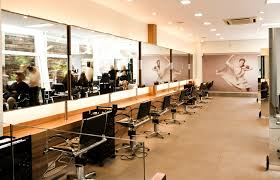
\includegraphics[width=0.8\textwidth]{images/salaoImagem.jpg}
		\caption{teste figura 1}
		\label{fig:imagem}
	\end{figure}
	
	mesmo usando uma hospedagem gratis (AWS), precisamos pesquisar uma paga para colocar na tabela de custos
	
	\section{Custos}
	
	\input{tabela-custos}
	
	\section{Receitas}
	\section{Cenário realista}
	\section{Cenário Otimista}
	\section{Cenário Pessimista}
	\cite{babel}
	% ---------------------------------------------------------------
	
	\chapter{Considerações Finais}
	\section{Dificuldades, escolhas e Descartes}
	\cite{ibge1993}
	% ----------------------------------------------------------
	
	ver documento "abntex2-modelo-include-comandos" para dicas e tutoriais de como fazer tabelas, graficos, quadros, inserir imagens e documentos externos etc aqui. 
	% ---
	
	%Página de referencias
	\renewcommand{\bibname}{Referências Bibliográficas} %renomeia o título da página de referencias
	\bibliography{referencias-bibliograficas}
	\bibliographystyle{abntex2-alf}
	\bibliographystyle{abntex2-num}
	
	
	% ----------------------------------------------------------
	% Glossário
	% ----------------------------------------------------------
	%
	% Consulte o manual da classe abntex2 para orientações sobre o glossário.
	%
	%\glossary
	
	% ----------------------------------------------------------
	% Apêndices
	% ----------------------------------------------------------
	
	% ---
	% Inicia os apêndices
	% ---
	\begin{apendicesenv}
		
		% Imprime uma página indicando o início dos apêndices
		\partapendices
		
		% ----------------------------------------------------------
		\chapter{exemplo 1}
		% ----------------------------------------------------------
		
		materiais desenvolvidos pelo próprio autor do trabalho
		
	\end{apendicesenv}
	
	% ----------------------------------------------------------
	% Anexos
	% Inicia os anexos
	
	\begin{anexosenv}
		
		% Imprime uma página indicando o início dos anexos
		\partanexos
		
		% ---
		\chapter{exemplo 1}
		matérias de outras fontes que não o próprio autor do trabalho
		
	\end{anexosenv}
	
	%---------------------------------------------------------------------
	% INDICE REMISSIVO
	%---------------------------------------------------------------------
	\phantompart
	\printindex
	%---------------------------------------------------------------------
	
\end{document}
